% chapters/01-prefix-sums.tex
\chapter{Prefix Sums}
\label{ch:prefix-sums}
\index{prefix sums}

\idea{Lemme ask one question: If I give you an array of size $n$, 
how do you compute the sum of elements from index $l$ to $r$?

A simple approach would be to iterate over the array and add up the elements. This would get 
messy(jk i know it's just nested loop) real quick as I give you more and more such 
queries. It would also slow things down. 
  
So the idea of prefix sum basically came in to solve this O(n) task in just O(1). }

\section{Core idea}
Given an array $a[1\ldots n]$, precompute $p[i]=\sum_{j=1}^i a[j]$ (fancy way of saying just add all prev elements to the current(i) one for all i's). Then any subarray sum $a[l..r] = p[r]-p[l-1]$ in $O(1)$ after $O(n)$ preprocessing.


A natural question to ask is: How did you come up to this formula?
My answer: Simple. $p[r]$ gives sum of all elements from 1 to r. But we only want from l to r. So we remove the sum of elements from 1 to l-1, which is $p[l-1]$. Hence the formula.

\example{
Suppose $a = [3,1,4,1,5]$. Prefixes: $p=[3,4,8,9,14]$. The sum from index 2 to 4 is $p[4]-p[1]=9-3=6$.
}



\textbf{Watch out for the edge case!} What if $l=0$? Then $l-1=-1$, and trying to access $P[-1]$ will cause an error.  
If $l=0$, the answer is just $P[r]$. You can handle this with a simple \texttt{if}-statement or a ternary operator.  

\section{Leveling Up: 2D Prefix Sums}
This same idea works for 2D grids! Imagine you need the sum of a rectangular area in a matrix.  
We can build a 2D prefix sum grid, $P$, where $P[i][j]$ is the sum of the rectangle from $(0,0)$ to $(i,j)$.  

To get the sum of a rectangle with corners at $(r_1, c_1)$ and $(r_2, c_2)$, we can use the Principle of Inclusion-Exclusion. It looks a little scary, but it's really simple when you think about it:
\[
\text{sum} = P[r_2][c_2] - P[r_2][c_1-1] - P[r_1-1][c_2] + P[r_1-1][c_1-1]
\]

Visually, you're taking the big rectangle from the origin ($A+B+C+D$), subtracting the parts you don't need ($B+A$ and $D+A$), and then adding back the corner ($A$) that you subtracted twice.

\begin{figure}
    \centering
    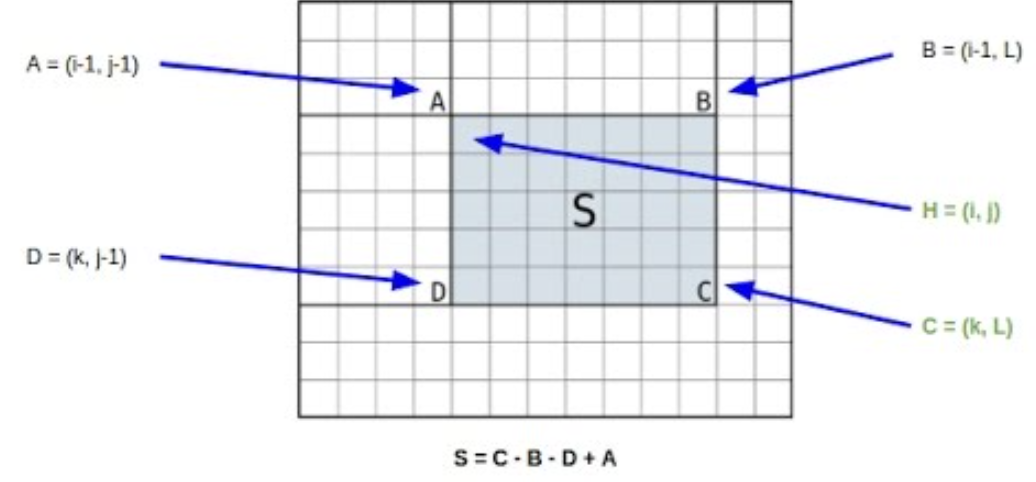
\includegraphics[width=0.6\textwidth]{figures/01-prefix-sums/2d_sum.png}
    \caption{2D Prefix Sums. Graphic taken from Arabic Competitive Programming YouTube Channel.}
\end{figure}

\section{Pro Moves: Weighted Prefix Sums}
Okay, what if the problem is weirder? Let's say you need a weighted sum like this:
\[
\text{need} = 1 \cdot A[l] + 2 \cdot A[l+1] + 3 \cdot A[l+2] + \dots + (r-l+1) \cdot A[r]
\]

A simple prefix sum won't work directly. This is where a key tip comes in handy: \textbf{If possible, try to write the problem as an equation}.  

The required sum can be written as:
\[
\sum_{i=l}^{r} (i-l+1) \cdot A[i]
\]

Let's split that up:
\[
\sum_{i=l}^{r} i \cdot A[i] \;-\; \sum_{i=l}^{r} (l-1) \cdot A[i]
\]

Pulling the constant $(l-1)$ out of the second term gives us:
\[
\left( \sum_{i=l}^{r} i \cdot A[i] \right) - (l-1) \left( \sum_{i=l}^{r} A[i] \right)
\]

Look at that! We've turned one tricky problem into two manageable ones:

\begin{enumerate}
    \item $\sum_{i=l}^{r} A[i]$: This is just a standard range sum! We can solve this with our basic prefix sum array, let's call it \texttt{P\_normal}.
    \item $\sum_{i=l}^{r} i \cdot A[i]$: This is a weighted sum. We can precompute another prefix sum array for this! Let's call it \texttt{P\_weighted}, where 
    \[
    \texttt{P\_weighted[i]} = \sum_{k=0}^{i} k \cdot A[k].
    \]
\end{enumerate}

Now the query can be solved in $O(1)$ using our two precomputed arrays. How cool is that?!

\section{The Ultimate Combo: Prefix Sums + Hash Maps}
Let's tackle another classic problem: Find the number of contiguous subarrays with an equal number of 0s and 1s. \textbf{Leetcode 525: Contiguous Array}

Try to solve it on your own first! If you're stuck, read on.

Here's a common trick people generally use: \textbf{Let all the 0s be $-1$s}.  

Now, a subarray with an equal number of 0s and 1s is a subarray whose elements \textbf{sum to 0}.  

So the problem is now "find all subarrays that sum to 0". We can use prefix sums for this! 

One more thing to notice is that a subarray from index $j+1$ to $i$ has a sum of 0 if:
\[
P[i] - P[j] = 0 \;\;\Longrightarrow\;\; P[i] = P[j]
\]

This means we're looking for pairs of indices where the prefix sum is the same. A hash map is the perfect tool for this. Now that the logic is clear, you can ask ChatGpt to help you out with code.

This combination of a clever trick ($0 \rightarrow -1$), prefix sums, and hash maps solves the problem in a single $O(n)$ pass.  

\section{Code Corner}
A quick tip for reading input:
\[
\texttt{for (auto \&it : v) cin >> it;}
\]

Refer to the appendix for more details.



\index{prefix sums!Practice problems}
\section{Practice problems}
\problem{Easy: Maximum Population Year (Leetcode 1854)}
\problem{Easy: Forest Queries | CSES}
\problem{Medium: Subarray Sums II | CSES}

% end chapter
